\subsection{Probabilistic models}
In many cases the features follows a certain distribution. By using the information in the distribution it is possible to filter out outliers and determine how likely it is that the point belongs to a certain class. This can be very powerful since we not blindly put a sample in a class but also get information about the likelihood. This of course demands that a qualified guess of the distribution can be made. 
By using the probability for a given sample, given a certain class $P(x|C)$. Iteration over the the different classes, it is possible to decide were to classify the sample, and how certain we are of this decision. This is illustrated in figure \ref{fig:disex} 

\begin{figure}[H]
\centering
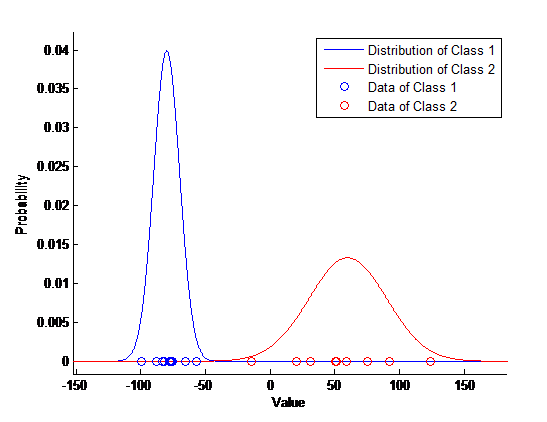
\includegraphics[scale=0.8]{billeder/DisEx}
\caption{Distributions of 2 Classes}
\label{fig:disex}
\end{figure}

\subsubsection{Discriminative Model}

Instead of asking what the probability of the sample, given the class is $P(x|C)$, the conditional probability can be used. That is the probability of a class, given a sample $P(C|x)$. This can be found using Bayes rule:
\begin{equation}
 P(C|x)=\frac{P(x|C)P(C)}{P(x)}
\end{equation}
This kind of model is called a discriminative model, and is used for modelling the dependence of an unobserved class $C$ on an observed variable $x$. This will for the Gaussian distribution be a sigmoid function. Using this model to classify it is no longer able to tell about the probability of a sample not being in any class, but on the same time also simplifies the classifier a lot. Compared to the linear classifier the discriminative classifier are able to create a mouth sharper decision bound. If the sharper decision bound is the goal then a easer approach is to estimate the optimal sigmoid for separation of classes directly. This can be done by optimizing a soft-max function to separate the classes. The soft-max function is expressed as: 
\begin{equation}
\label{eq:softmax}
 y_k(\textbf{w}_k,\textbf{x})=\frac{e^{\textbf{w}_k \textbf{x}}}{\sum\limits_{k=1}^K e^{\textbf{w}_k \textbf{x}}}
\end{equation}
Comparing this to the previous probabilist function we can assume that:
\begin{equation}
\label{eq:baseassmution}
 P(t|\textbf{w},\textbf{x}_n) = p_n^t (1-p_n)^{1-t} , t \in [0,1] 
\end{equation}
Here we see how likely it is that the class vector t, is correct given data point x, and some weights w in the soft-max.  Where t is the class vector, that indicates which class the data point x is part of.  The $p_n$ is given by: 
\begin{equation}
 p_n = P(C| \textbf{w}, \textbf{x}_n) = y(\textbf{w},\textbf{x}_n)
\end{equation}
The challenge is now to find the optimal weights $w_k$, for each class, to create the best classifier. This can be done by combining the two equations \ref{eq:softmax}, \ref{eq:baseassmution} to create a non linear optimisation problem.
\begin{equation}
 L(w) = \log{\prod\limits_{i=1}^N y(\textbf{w},\textbf{x}_i)^{\textbf{t}_i} ( 1-y(\textbf{w},\textbf{x}_i))^{1-\textbf{t}_i}}
 = \sum\limits_{i=1}^N t_i\log{y(\textbf{w},\textbf{x}_i)}+(1-\textbf{t}_i)\log({1-y(\textbf{w},\textbf{x}_i))}
\end{equation}
This can be solved by many different optimizations strategies. By optimizing this for each class we will find the optimal weights for the soft-max class separator in equation \ref{eq:softmax}.\\

In the speaker recognition case a soft-max function has been used to create a discriminative model, that are able to separate the classes as described above. A full probabilistic model using the $P(x|C)$ approach, has also been attempted by using a Gaussian mixture model. This is described in the section: \ref{sec:EMGMM}. In this analysis it is assumed that the data is Gaussian distributed. This assumption is made by looking at the histogram of the features. This is shown on figure \ref{fig:featurehist}.

\begin{figure}[H]
\centering
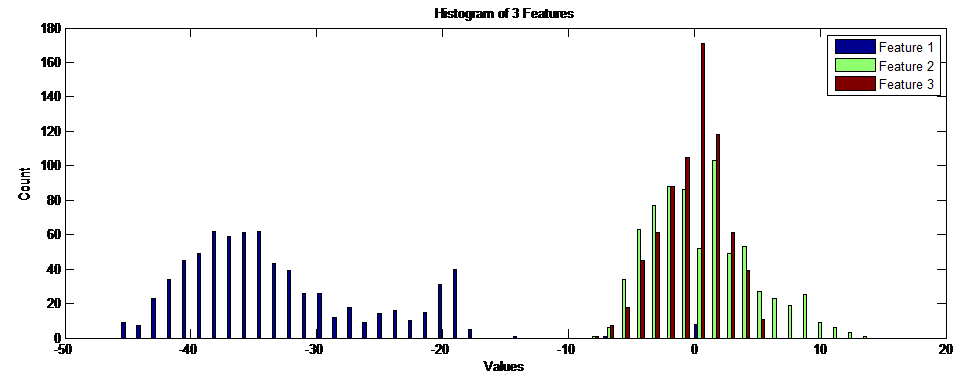
\includegraphics[scale=0.6]{billeder/histoffeature}
\caption{Histogram of 3 features}
\label{fig:featurehist}
\end{figure}

By running the optimizing the soft-max function a model is found that are capable of separating the test set in the three classes, whit a 21.58 \% error rate. The results can be seen in table \ref{tab:resultTableProp}. 

\begin{table}[h]
\centering
\begin{tabular}{ll}
\hline
Total Error   & 21.58 \% \\ \hline
Nicolai Error & 24.27 \% \\
Rasmus Error  & 10.68 \% \\
Rune Error    & 29.77 \% \\ \hline
\end{tabular}
\caption{Discriminative Model Results}
\label{tab:resultTableProp}
\end{table}

The results indicate that Rune is the one there is hardest to classify. Even though some samples are classified wrong, the majority of samples is correct classified. This makes this method valid for speaker recognition. \\
\ \\

\fxnote{have awesome glud billed .}

%------------------------------------------------